\documentclass[../main.tex]{subfiles}
%\graphicspath{{\subfix{./images/}}} %Does not work...

\begin{document}
\section{Design Process and Potential Solutions}\label{designProcess}

\subsection{Design Synthesis Process}
Throughout the synthesis of potential designs, a cyclical and iterative design process was followed. Although this process pairs very well with almost any problem, the team found it to be the most useful design synthesis process. The cyclical nature of said process allows further definition of the project scope in alignment with the overall problem and mission statement of the team.\par
In the first phase, the Ask and Identify phase, we were tasked at identifying the problem at hand and creating a problem statement and finding all relevant background information on it. We identified relevant questions to look at to understand our problem statements, and worked together to create a problem statement. \par
In the second phase, the Research the Problem phase, we were in charge of conducting all relevant research and meeting with stakeholders. We conducted interviews with them to gather knowledge on the subject and to frame out research better. We then compiled all of our research in a literature review in our paper to reference later. \par
In the third phase, the Imagine Possible Solutions phase, we conducted various brainstorming sessions to generate possible solutions for our problem. Once we generated these solutions, we narrowed them down to a few refined ones, that could be serious candidates for our final project. We discussed the ideas with others, specifically stakeholders, to also make sure we were on the right track. \par
\newpage

In the fourth phase, the Select Idea/Prototyping phase, we will create a decision matrix to finalize a solution. Then, we will create a rapid prototype and test with potential users or experts. \par
In the fifth and final phase, the Build and Test phase, we will develop a risk assessment matrix and cost-benefit analysis for your project. We will also finalize our prototype and prepare a final project presentation. \par

\newpage
\subsection{Proposed Solutions}
\noindent\textbf{Solution \#1:}\newline
\indent One of our potential solutions offers fully-electric hangars -- working with FBOs -- to private businesses with an emphasis on cargo companies like Amazon, UPS, and FedEx. These companies have already set carbon-neutral goals as early as 2040 (Amazon announced this in 2019 and FedEx in 2021), so there is a large EA market in their industry. And since funding is a major EA issue, these companies could even sponsor the development from the get-go to ensure their specific needs are met. As discussed in our research, the power-density limitations of current battery technology would limit the cargo capabilities to small/middle weight deliveries. This would allow the companies to use EAs from their HUB airports to smaller regional locations -- which would already be carrying comparatively smaller loads shorter distances. The solution would offer personalized tarmac routes for EAs and prioritization for such aircraft. This would be a major appeal to these businesses competing to offer the quickest delivery services in our new age of "next-day delivery." \par
\begin{figure}[h!]
    \fbox{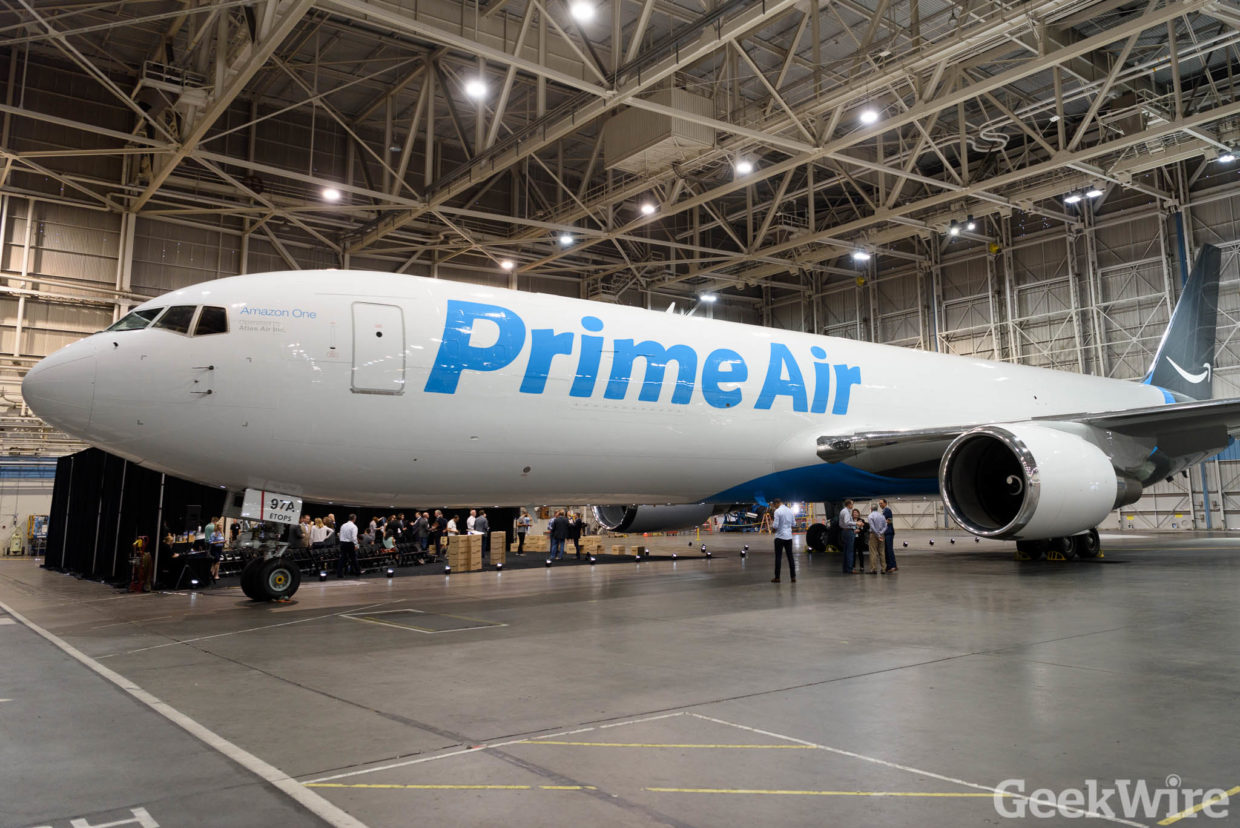
\includegraphics[width=0.5\textwidth]{amazon_hangar.jpg}}
    \centering
    \caption{An existing hangar devoted to Amazon Prime diesel planes}
    \centering
\end{figure}
\newpage
\noindent\textbf{Solution \#2:}\newline
\indent A different solution to consider is utilizing a universal hanger. Instead of having a privately owned hanger, there would be one that all companies would use to charge their plane, which in turn puts less demand on infrastructure. For private flights, there would be a universal charger or a type of adapter that any plane can use to charge their plane, available at the hanger. This creates an easy way for any private electric plane to recharge at any hanger. There would be less stress on infrastructure because there would be no need to personalize different hangers and less cost as well since they would all be the same, within the same plugs and adapters. \par
\begin{figure}[h!]
    \fbox{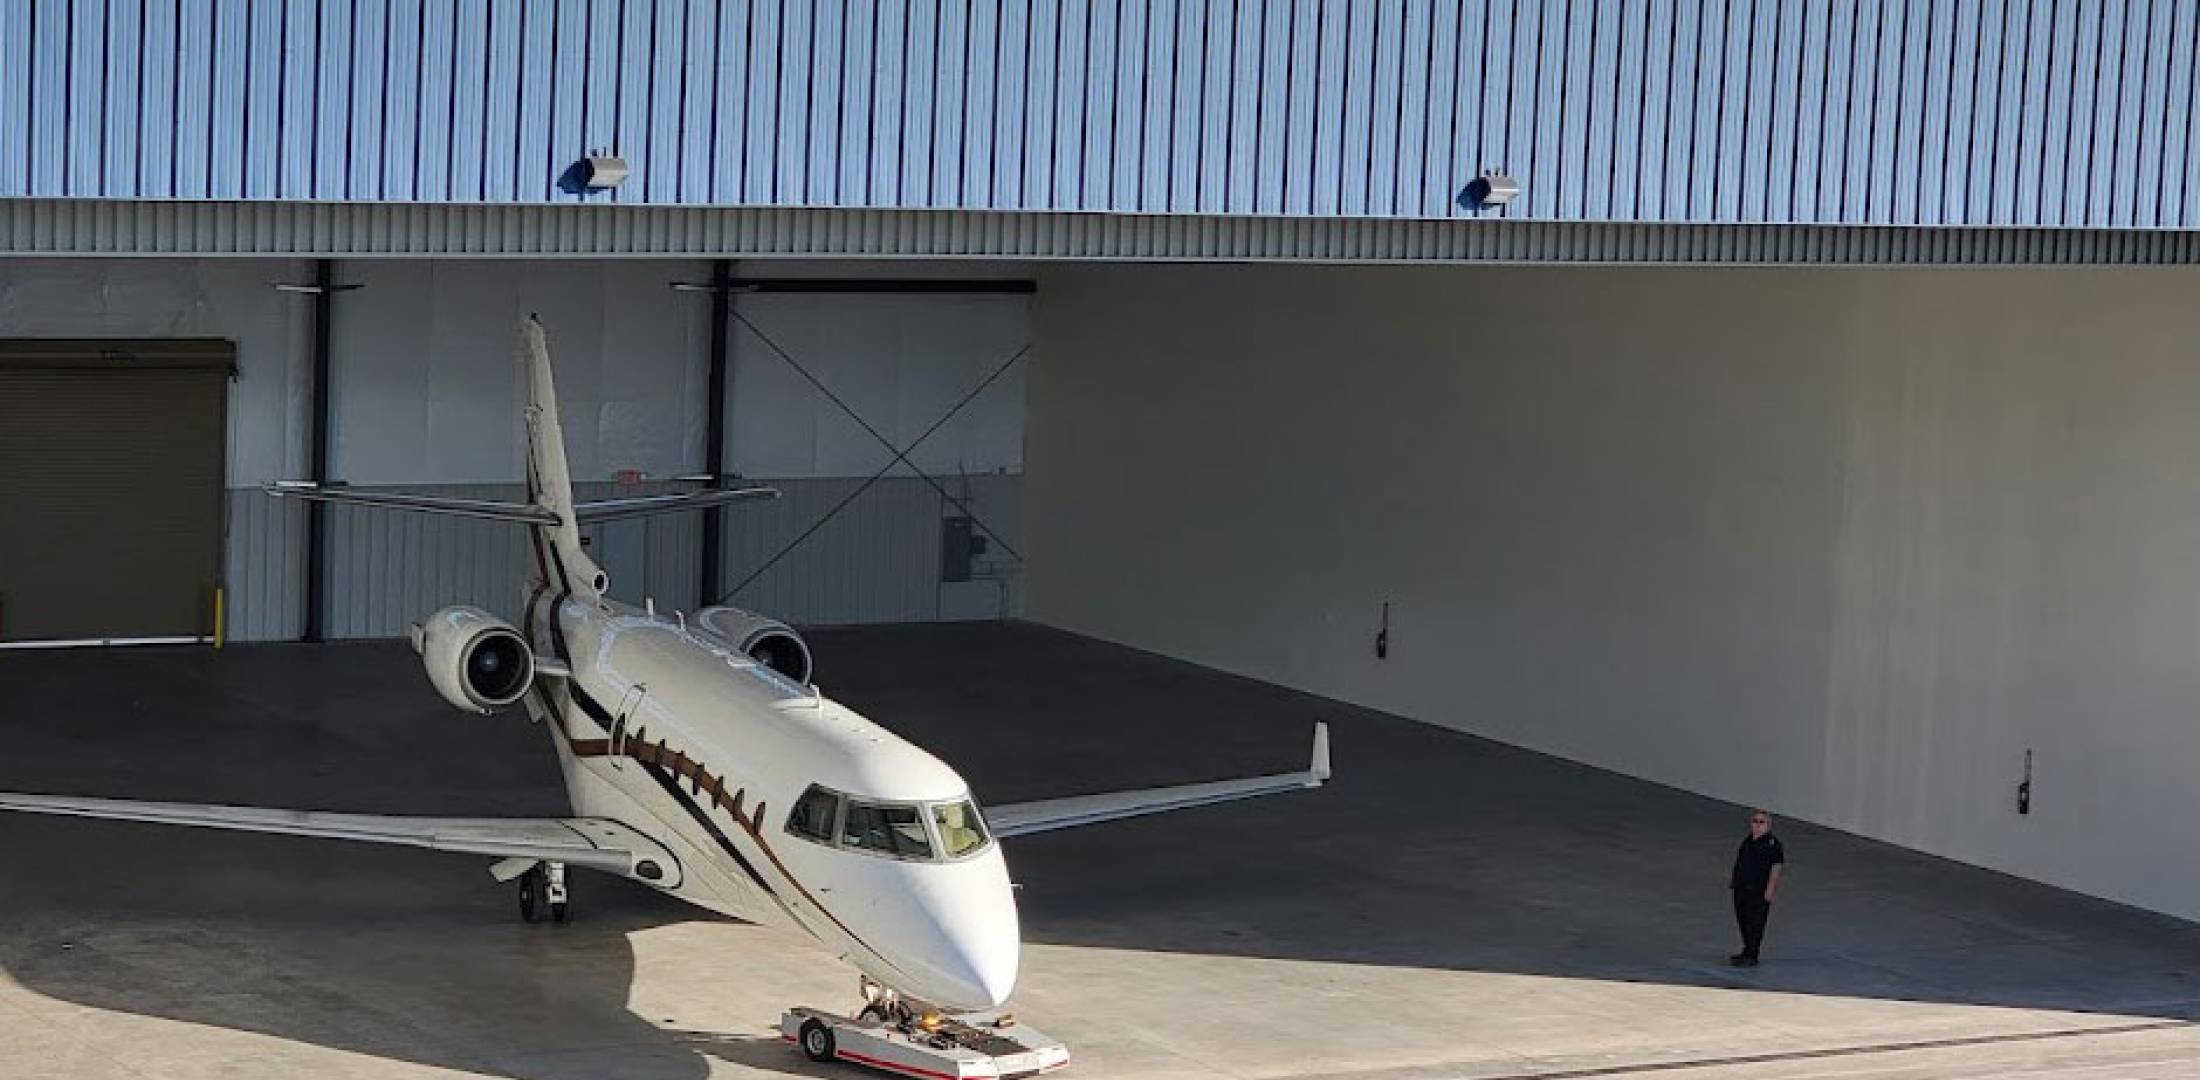
\includegraphics[width=0.8\textwidth]{hanger.jpeg}}
    \centering
    \caption{A privatized aircraft hanger}
    \centering
\end{figure}

\newpage
\noindent\textbf{Solution \#3:}\newline
\indent This solution mainly deals with the big question: where will this project receive funding? Even if technology gets to a point where electric aircrafts can be easily implemented into society, the question is who will pay for it, and how. Just as farm equipment can receive a tax cut to encourage farming, government subsidized implementation of green power generation systems such as turbines or solar panels could be used to encourage the market for electric vehicles. The long-term idea is this: If airports get a tax cut for using a certain percentage of electricity from natural resources, they can offer cheaper charging rates and services which will attract customers, therefore creating a bigger market for electric aircrafts.  \par
\begin{figure}[h!]
    \fbox{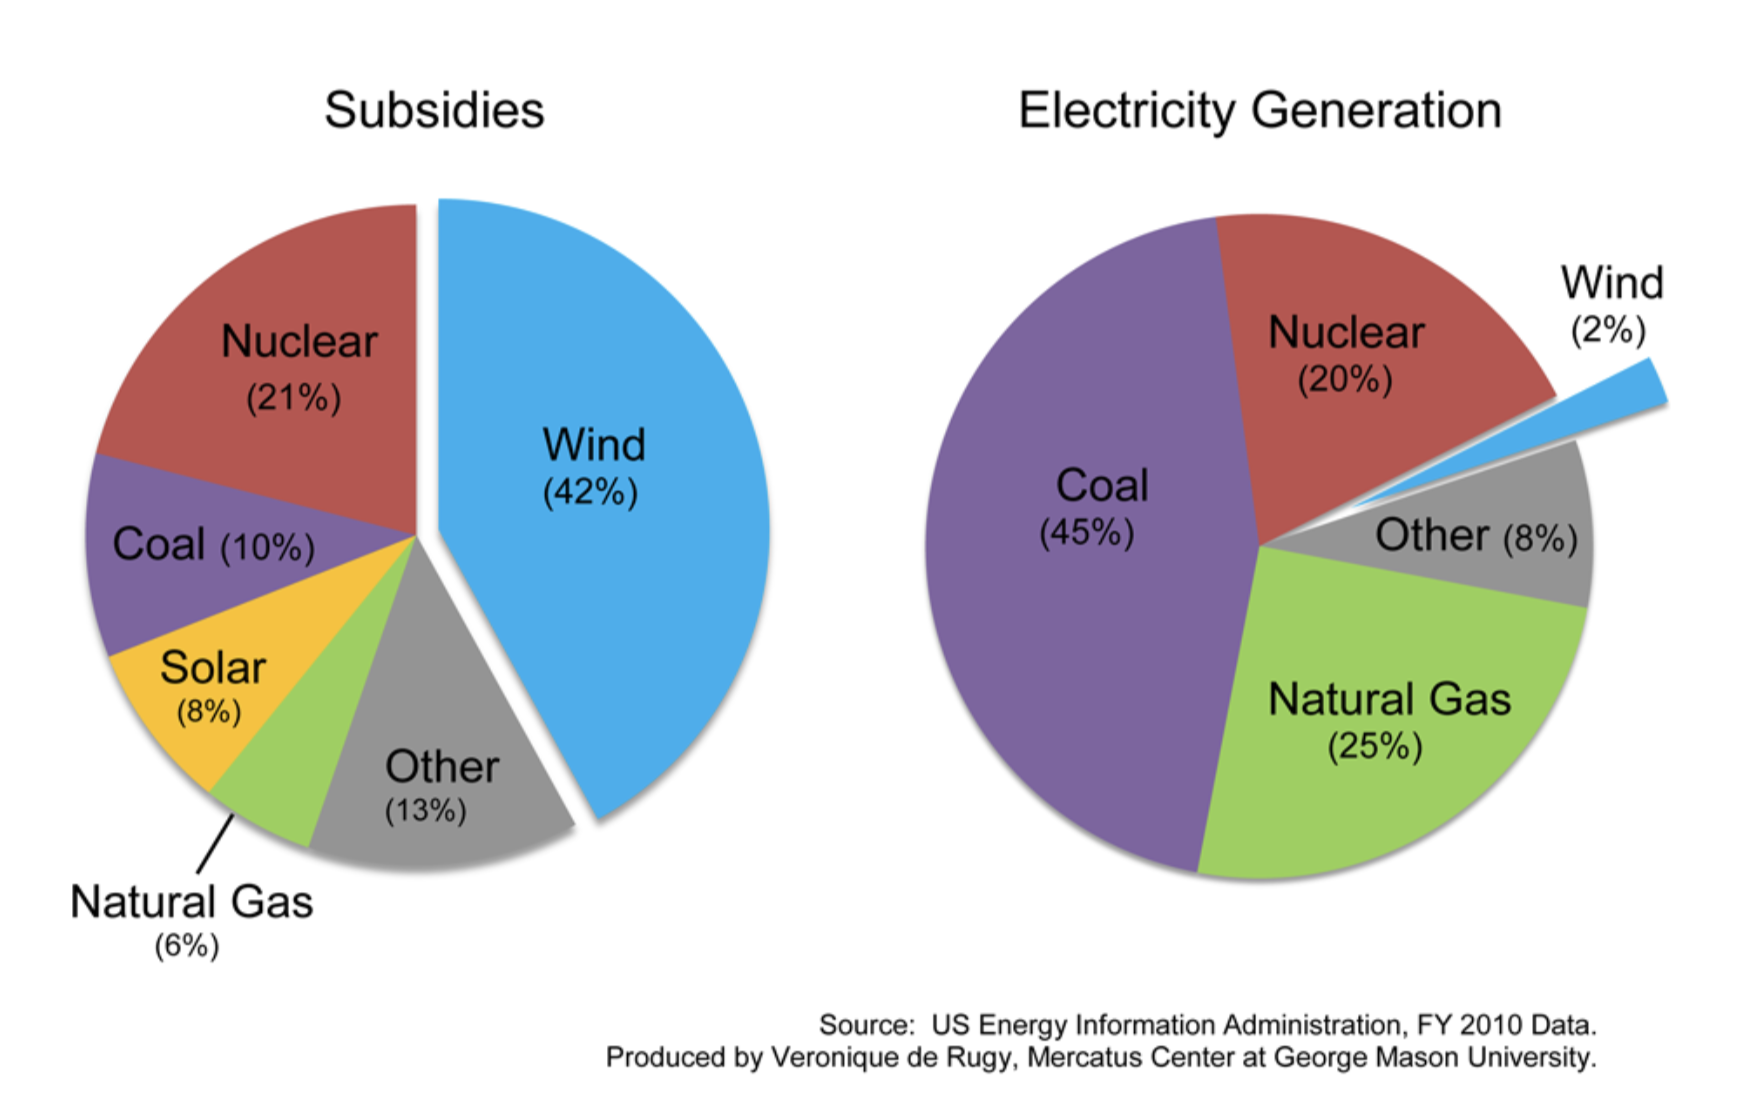
\includegraphics[width=0.6\textwidth]{graph.png}}
    \centering
    \caption{Renewable Energy Subsidies and Electricity Generation Pie Chart}
    \centering
\end{figure}

\newpage
\noindent\textbf{Solution \#4:}\newline
\indent Perhaps a bit more technical, the next potential solution centers itself on the necessary electrical storage, generation and geographical demands for an airport (or an FBO) to provide energy to aircraft. Using low-glare panels and performance predictions for both battery power density and panel efficiency, a model can be developed showing the amount of square yards required to charge a small to regional aircraft. This model would then be applied to a site, demonstrating a variety of methods by which power is generated, stored, and distributed. This solution hopes to provide maximum space efficiency, utilizing the existing geography at the airport as a dual-use zone.\par
\begin{figure}[h!]
    \centering
    \fbox{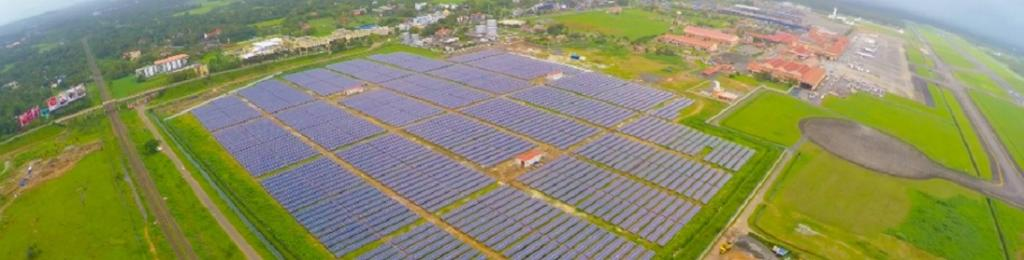
\includegraphics[width=0.8\textwidth]{solarArray.jpg}}
    \caption{A large solar generation array}
    \centering
\end{figure}

\newpage
\noindent\textbf{Solution \#5:}\newline
\indent The implementation of large scalable energy storage and power generation systems is a key factor in reducing the carbon footprints airports carry. With the great increases in market demand for electric planes, so comes a greater demand for power storage -- something not currently considered in large-scale generation systems. Effective implemenation of both a power generation and storage system has a twofold benefit for capitol investment. The first obvious benefit is that, obviously, there is capacity to charge EA. The second and more understated benefit is that if EA do not reach the anticipated market growth, an effective power storage system can be used to supply power to additional markets. This is especially adventageous when keeping in consideration that airports are largely a government-subsidized entity, and thusly have large capitol resources available for such a proposed infrastructure project.
\begin{figure}[h!]
    \fbox{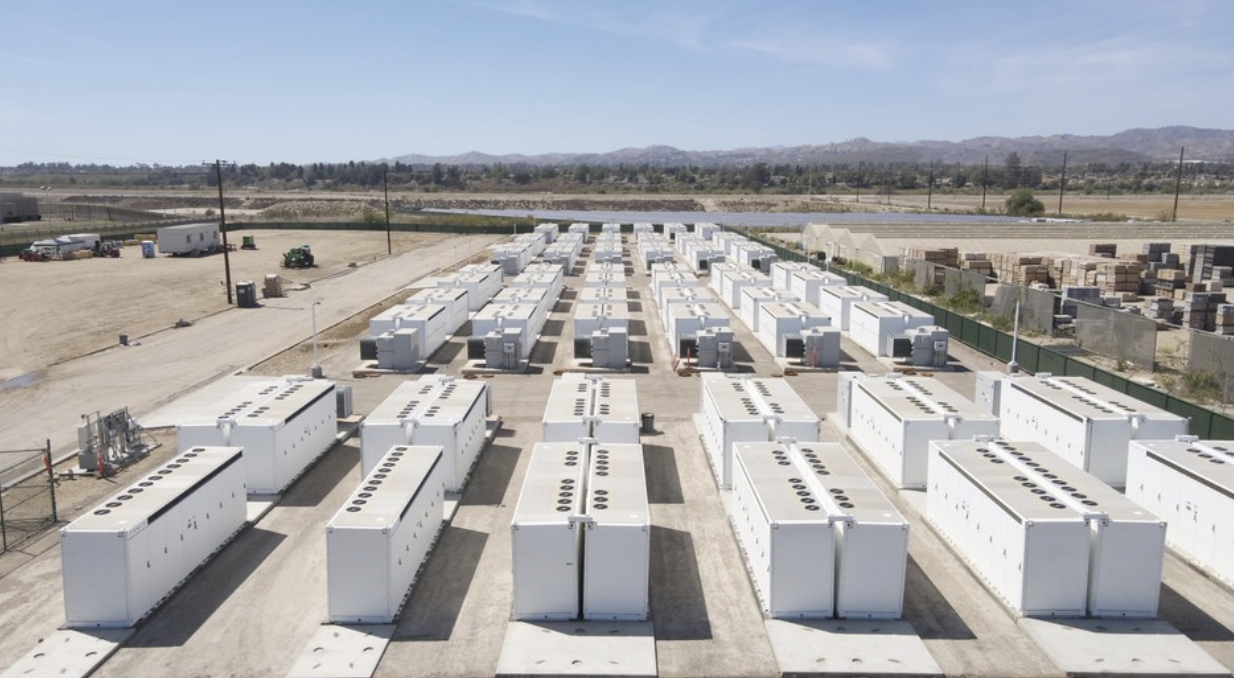
\includegraphics[width=0.7\textwidth]{large-scale.png}}
    \centering
    \caption{Large Scale Energy Storage}
    \centering
\end{figure}
\end{document}